\documentclass[conference]{IEEEtran}
\IEEEoverridecommandlockouts
% The preceding line is only needed to identify funding in the first footnote. If that is unneeded, please comment it out.
\usepackage{cite}
\usepackage{amsmath,amssymb,amsfonts}
\usepackage{algorithmic}
\usepackage{graphicx}
\usepackage{textcomp}
\usepackage{xcolor}
\usepackage{ctex}
\usepackage{fontspec}
\usepackage{listings}
\usepackage{algorithm}

\def\BibTeX{{\rm B\kern-.05em{\sc i\kern-.025em b}\kern-.08em
    T\kern-.1667em\lower.7ex\hbox{E}\kern-.125emX}}
\begin{document}

\title{数字图像处理实践报告}

\author{\IEEEauthorblockN{黄润华}
\IEEEauthorblockA{\textit{中国海洋大学} \\
huangrunhua@stu.ouc.edu.cn}}

\maketitle

\begin{abstract}
本报告为数字图像处理课程中期实践报告,主要内容为图像目标检测。报告内仿真内容部分均采用Matlab编程语言实现,仿真软件环境为Matlab R2021b,设备处理器为Apple M1,运行内存为16GB。
\end{abstract}

\begin{IEEEkeywords}
    image enhancement, image denoising, side window filter, Wiener filter
\end{IEEEkeywords}

\section{实践内容}
图像中待检测目标包含有孔圆环、无孔圆环、矩形和直线。图像是二值图像,由于成像原因受到椒盐噪声的干扰。各几何图形之间没有重叠或接触(直线可以相交)。要求检测出图像中的各个目标,即给出:有孔圆环的圆心坐标和内外半径、无孔圆环的圆心坐标和半径、矩形的质心坐标和边长以及直线的参数。设计算法并编程实现上述自动检测。

\begin{figure}[htbp]
	\centerline{
		
\includegraphics[width=9cm]{1.png} 	
	}
	\caption{含椒盐噪声的待检测图像}
	\label{pic1}
\end{figure}

\section{图像检测算法}
本节给出本次利用Matlab进行图像识别所采用的算法。其中算法\ref{alg:sir}给出了对灰度图像中线段进行识别的算法。算法\ref{alg:circle}给出了对灰度图像中圆形图像进行识别的算法。需要注意的是,在进行圆形识别过程中需要人为划定一条大致的直线作为圆形半径的可选值。算法\ref{alg:circle}中$\sum_{xy}$表示对$x$与$y$进行轮换对称,即$d = \sqrt{(x_1 - x_2)^2 + (y_1 - y_2)^2}$。算法\ref{alg:tris}给出了灰度图像中矩形图像识别的算法。由于矩形的特殊性,在算法执行的过程中需要分别进行两次霍夫变换。
\begin{algorithm}[H]
    \caption{直线检测识别算法}\label{alg:sir}
    \begin{algorithmic}
    \STATE 
    \STATE \text{将图像转为灰度图像并加中值滤波去噪}
	\STATE \text{边界提取}
	\STATE \text{选择合适的参数利用hough进行霍夫变换}
	\STATE \text{存储所有识别的线段lines}
    \STATE \hspace{0.5cm}$ \textbf{FOR} \;\;i = 1: length(lines)$
    \STATE \hspace{1cm}\text{ 计算线段的长度 }
    \STATE \hspace{0.5cm}$ \textbf{END FOR}$
	\STATE \hspace{0.5cm}$ \textbf{FOR} \;\;i = 1: length(lines)$
    \STATE \hspace{1cm}\text{ 查找最长的三条线段并存储 }
    \STATE \hspace{0.5cm}$ \textbf{END FOR}$
    \STATE \hspace{0.5cm}$ \textbf{FOR} \;\;i = 1: N_s$
    \STATE \hspace{1cm} \text{利用.point1属性变量获取线段的起始点}
	\STATE \hspace{1cm} \text{利用.point2属性变量获取线段的终点}
	\STATE \hspace{1cm} \text{利用数学知识计算直线斜率与截距等参数}
    \STATE \hspace{0.5cm}$ \textbf{END FOR}$
    \end{algorithmic}
\end{algorithm}

\begin{algorithm}[H]
    \caption{圆形检测识别算法}\label{alg:circle}
    \begin{algorithmic}
    \STATE 
	\STATE \text{ 加载图像转为灰度图像并显示 }
	\STATE \text{ 利用drawline函数确定搜索圆的半径范围 }
	\STATE $\text{ 获取line的起始点 }(x_1, y_1)\text{与终点 }(x_2, y_2)$
	\STATE $\text{ 计算line的长度作为圆的直径 } d = \sqrt{\sum_{xy}(x_1 - x_2 )^2}$
	\STATE $\text{ 搜索半径范围为 } [\frac{d}{2} - 5, \frac{d}{2} + 5] \text{的圆}$
	\STATE \text{利用imfindcircles计算圆心与半径}
    \end{algorithmic}
\end{algorithm}

\begin{algorithm}[H]
    \caption{矩形检测识别算法}\label{alg:tris}
    \begin{algorithmic}
    \STATE 
    \STATE \text{将图像转为灰度图像并加中值滤波去噪}
	\STATE \text{边界提取}
	\STATE $ \textbf{FOR} \;\;i = 1: 2$
	\STATE \hspace{0.5cm}\text{选择合适的参数利用hough进行霍夫变换}
	\STATE \hspace{0.5cm} \text{存储所有识别的线段lines}
    \STATE \hspace{1cm}$ \textbf{FOR} \;\;i = 1: length(lines)$
    \STATE \hspace{1.5cm}\text{ 计算线段的长度 }
    \STATE \hspace{1cm}$ \textbf{END FOR}$
	\STATE \hspace{1cm}$ \textbf{FOR} \;\;i = 1: length(lines)$
    \STATE \hspace{1.5cm}\text{ 查找平行且最长的两条线段并存储 }
    \STATE \hspace{1cm}$ \textbf{END FOR}$
	\STATE $ \textbf{END FOR}$
    \STATE \text{合并两次霍夫变换得到的四条线段}
	\STATE \text{将接近的两个端点求取均值作为矩阵的顶点坐标}
    \end{algorithmic}
\end{algorithm}

\section{检测结果}
\subsection{直线检测结果}
\begin{figure}[htbp]
	\centerline{
		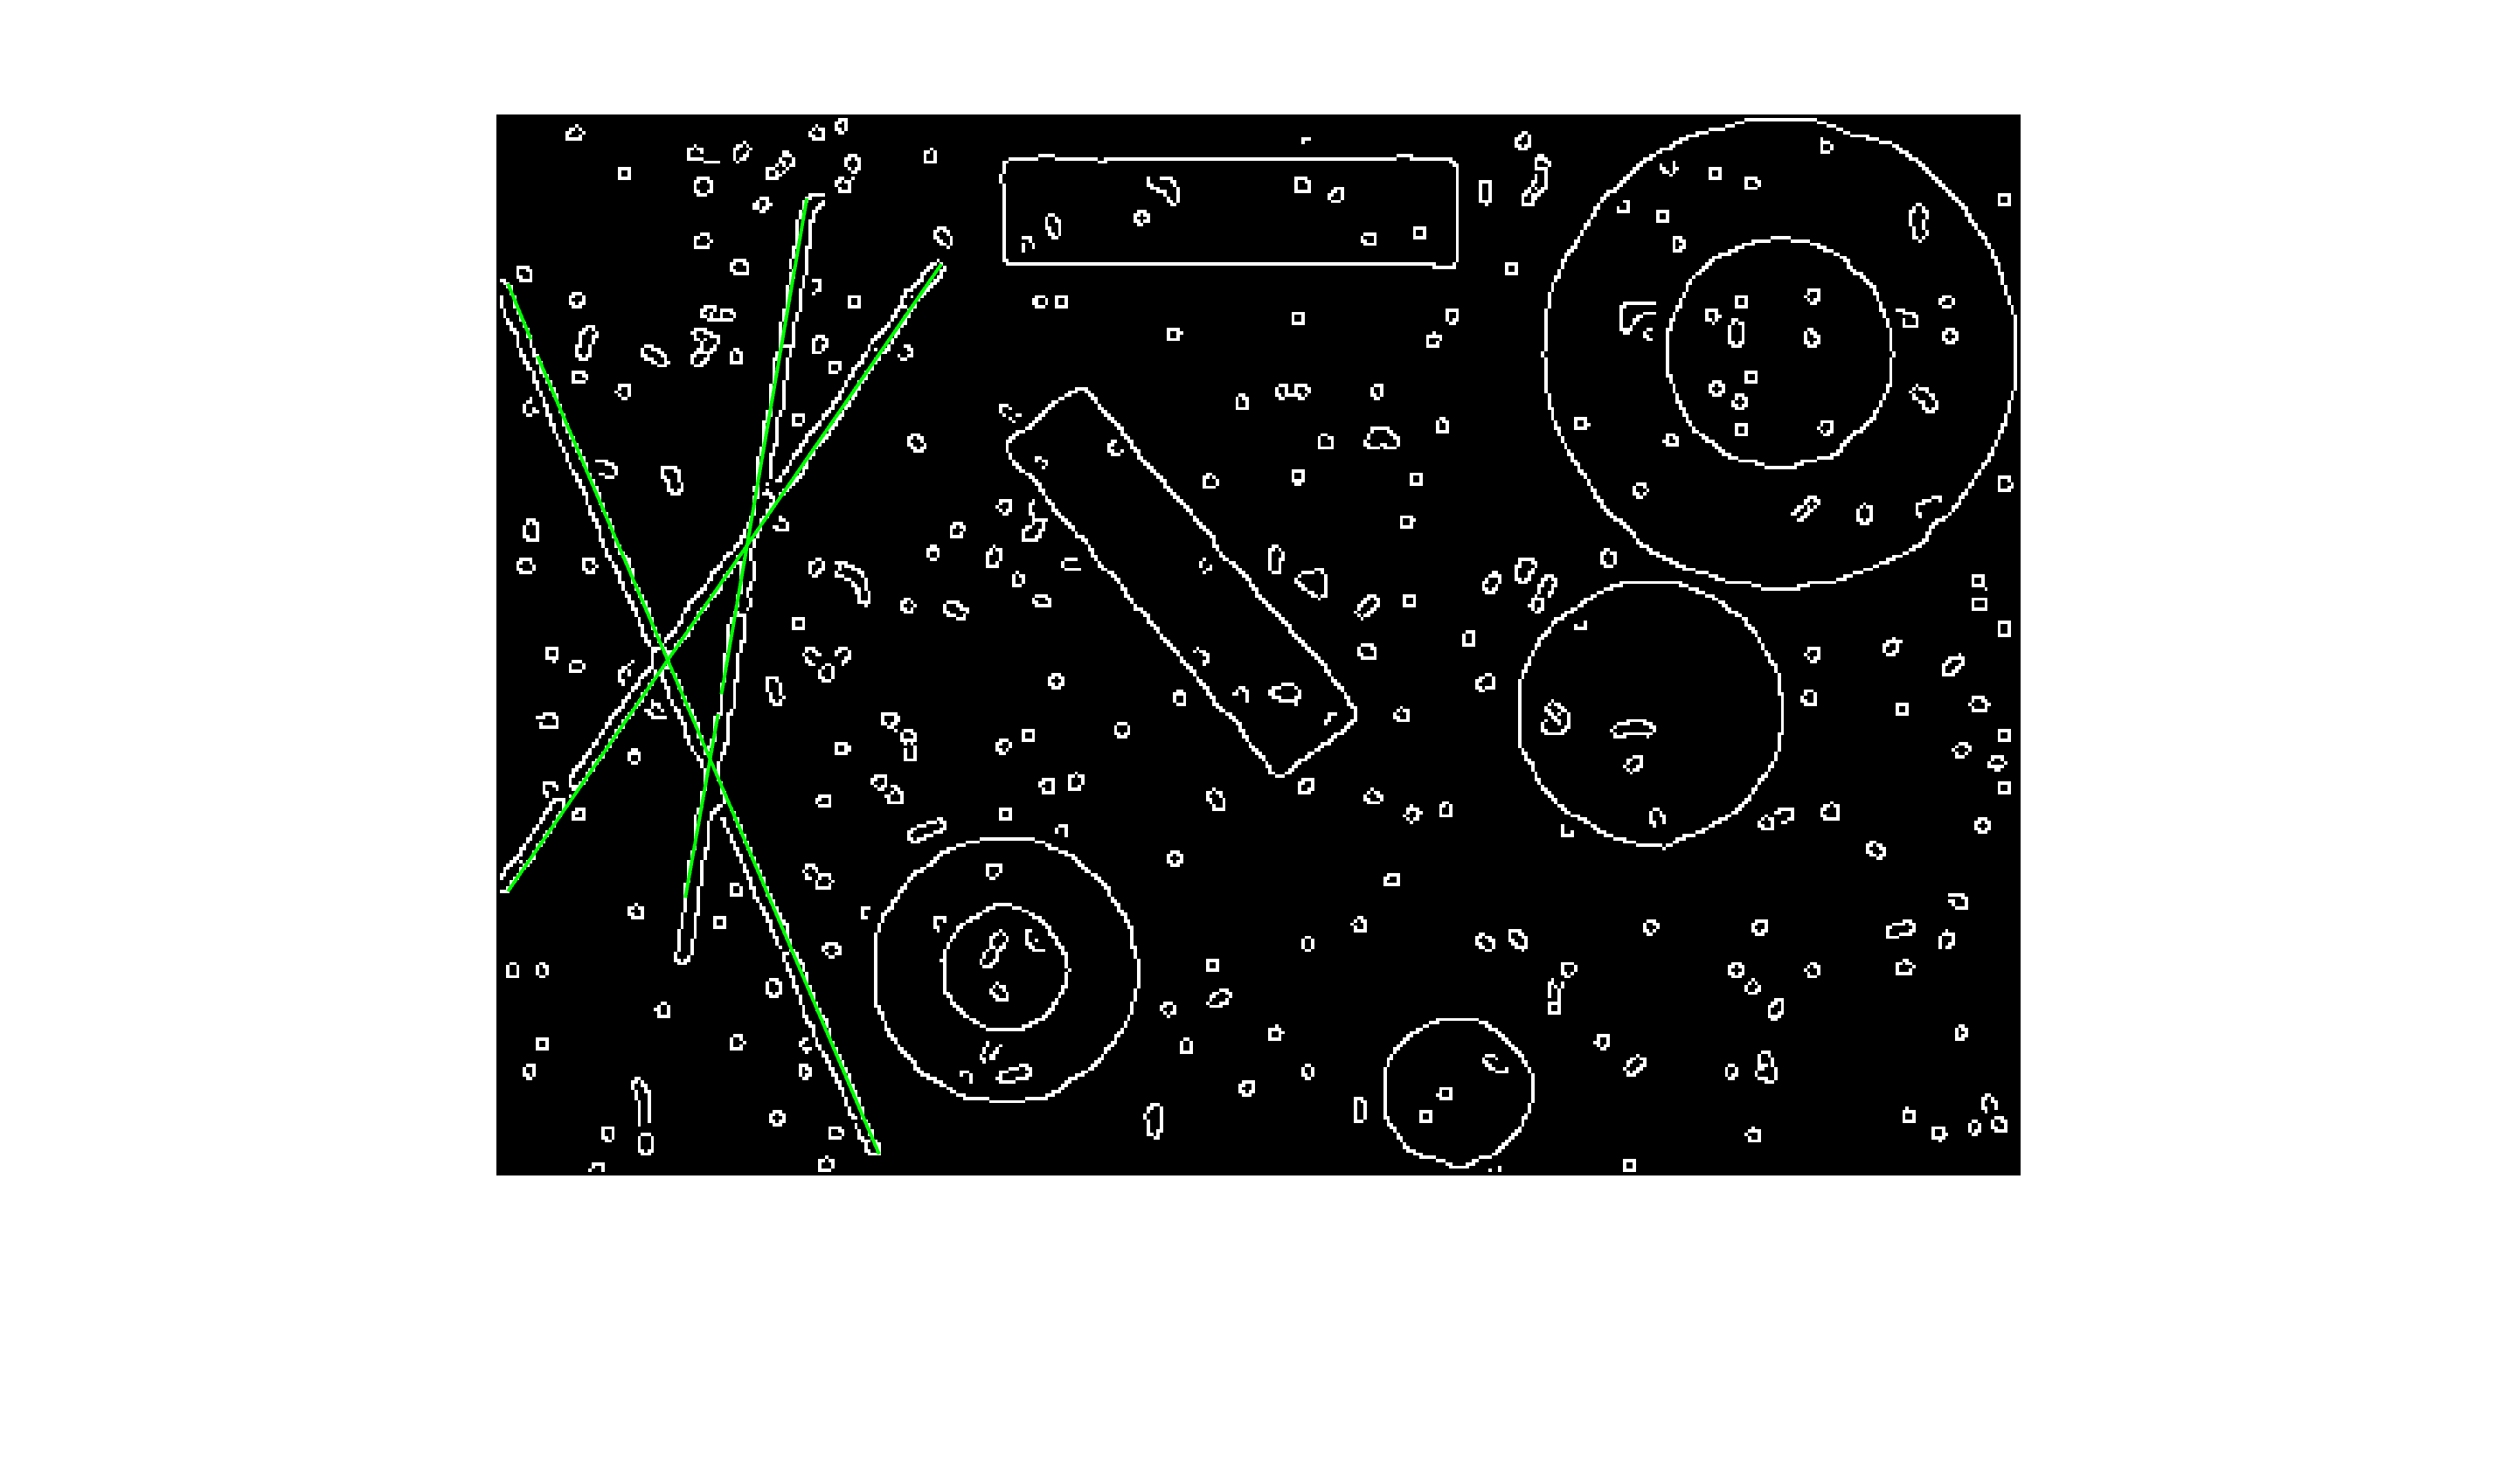
\includegraphics[width=9cm]{lines.png} 	
	}
	\caption{直线检测结果}
	\label{pic2}
\end{figure}
图片\ref{pic2}显示了对灰度图像中线段进行识别与检测的结果。表格\ref{table1}给出了三条线段的起始点与终点。

\begin{table}[htbp]
	\caption{线段检测结果}
	\label{table1} 
	\centering  
	\begin{tabular}{|c|c|c|}
	\hline
	线段 & 起始点 & 终点 \\
	\hline
	线段1 & (4, 52) & (117, 317) \\
	\hline
	线段2 & (95, 26) & (58, 239) \\
	\hline
	线段3 & (4, 237) & (136, 46) \\
	\hline
	\end{tabular}
\end{table}

\subsection{圆与圆环检测结果}
\begin{figure}[htbp]
	\centerline{
		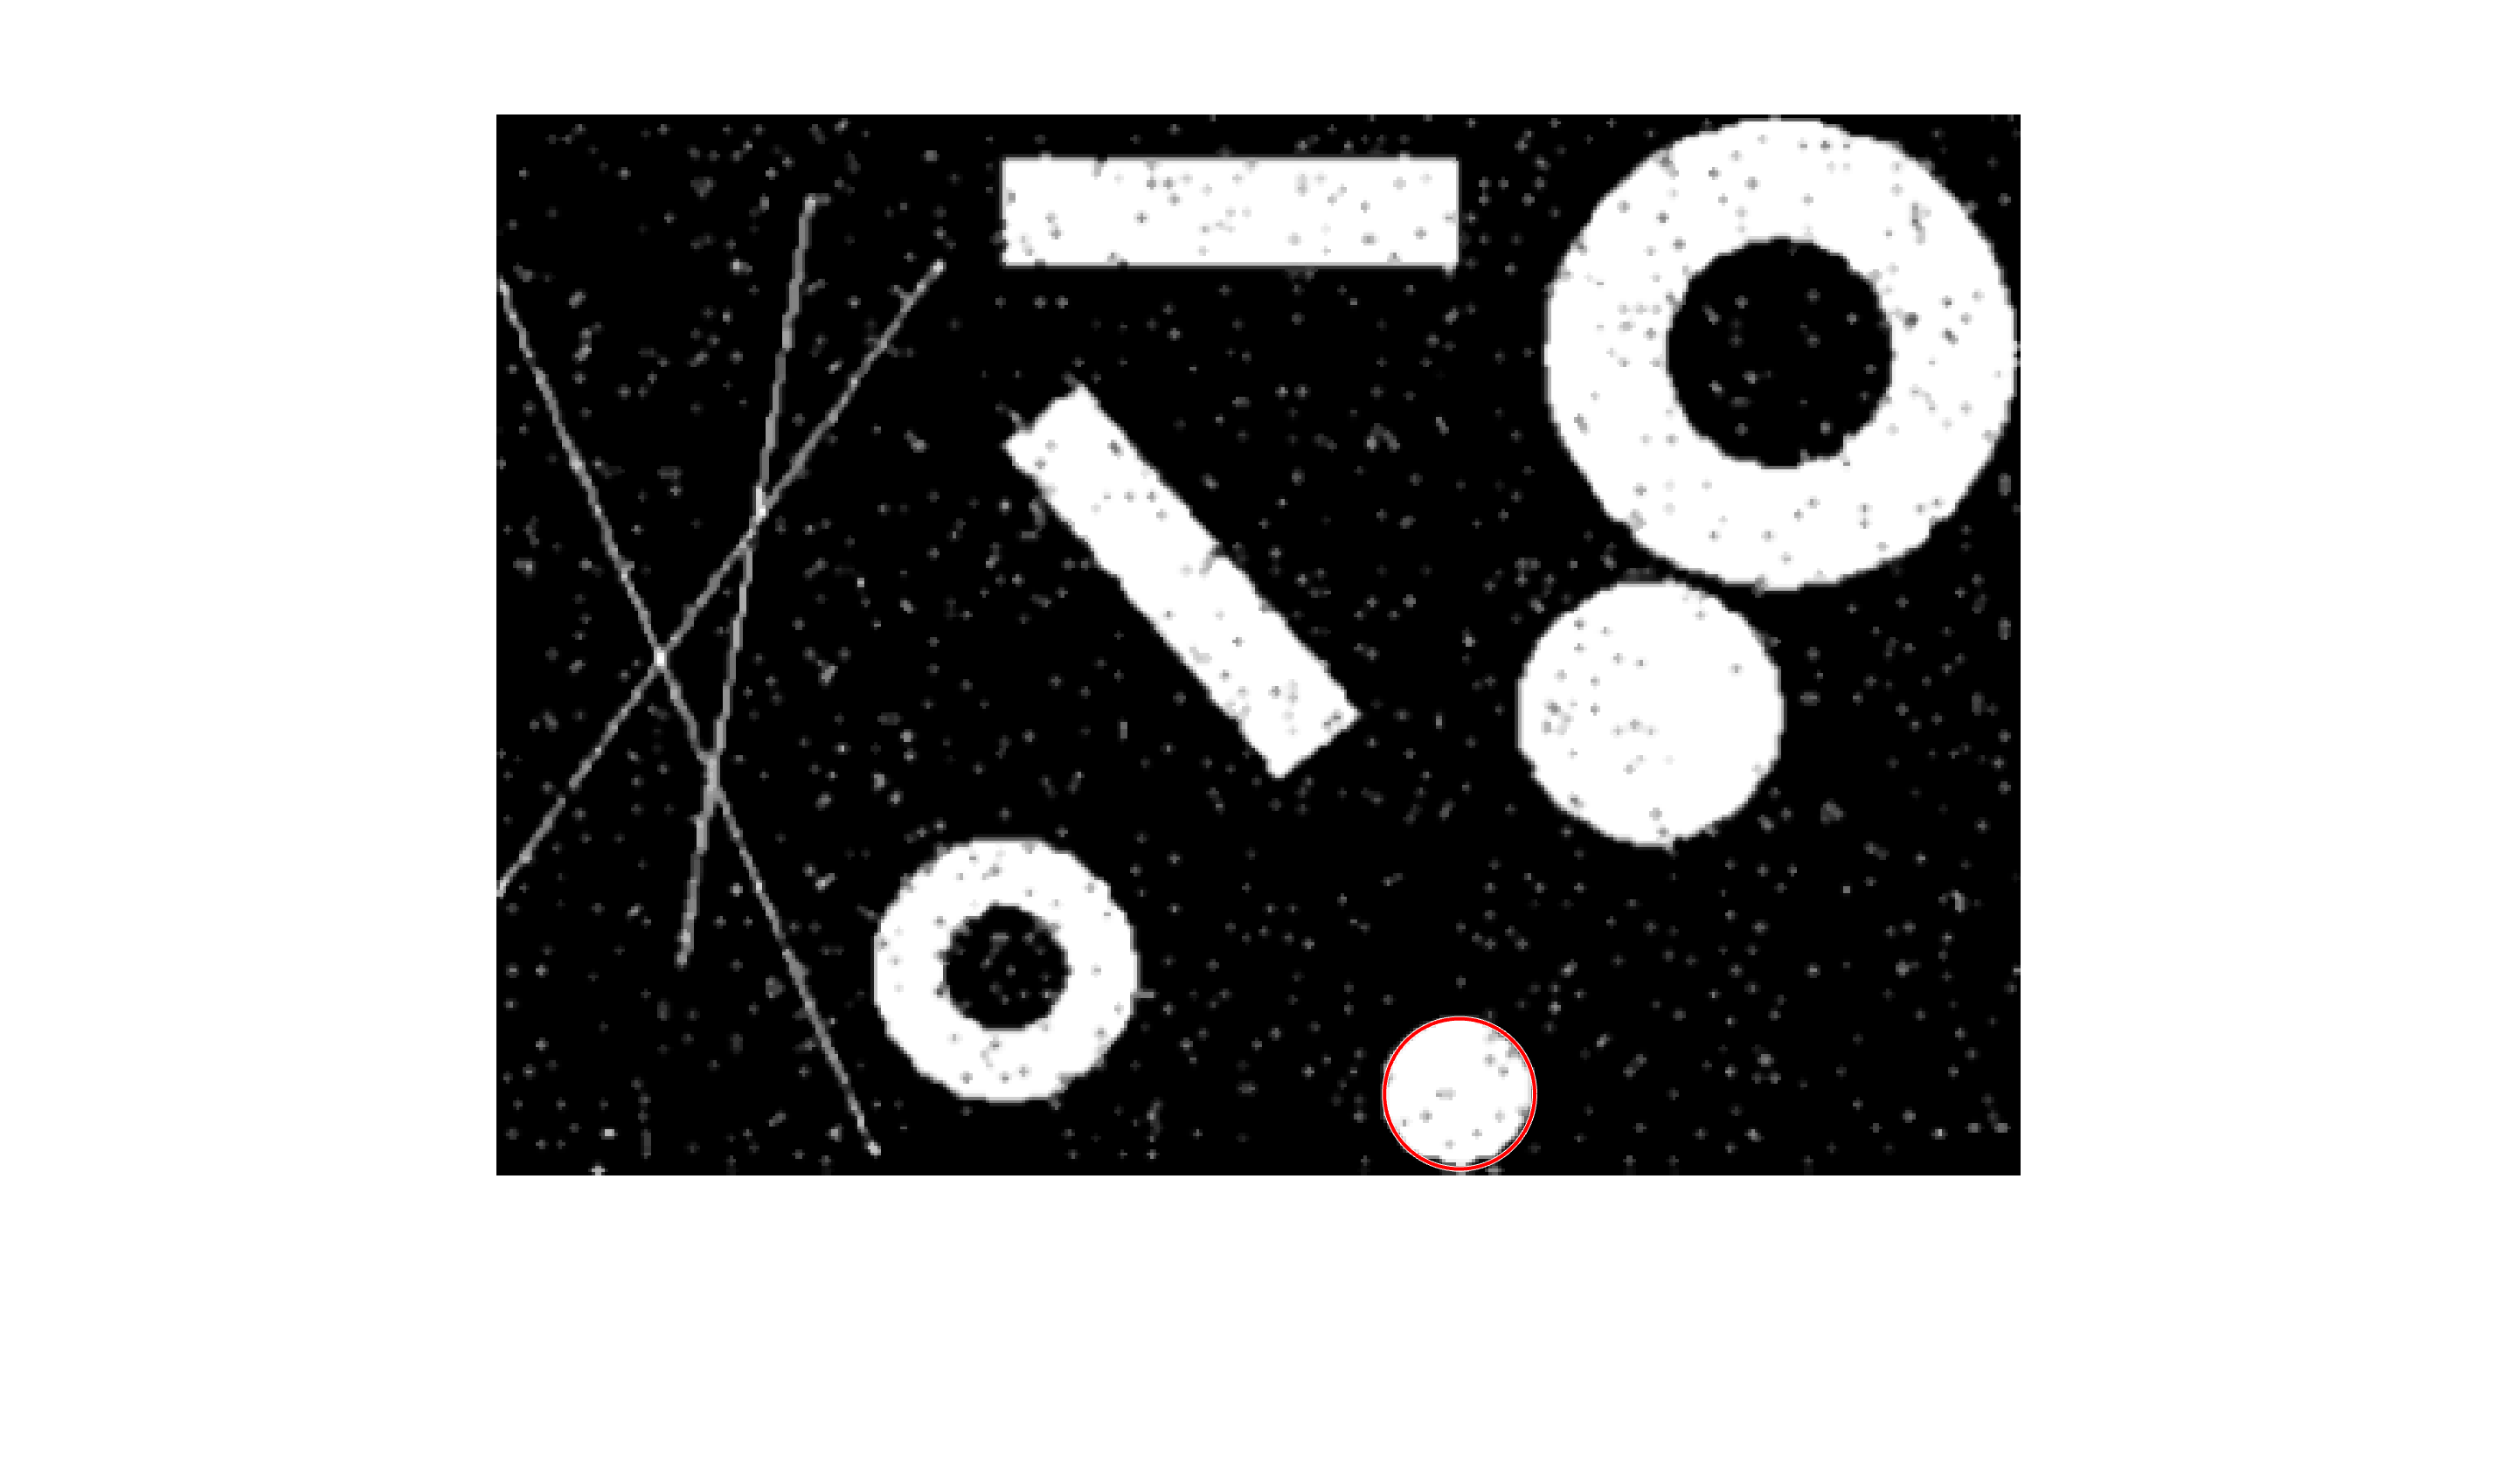
\includegraphics[width=9cm]{circle1.png} 	
	}
	\caption{圆与圆环检测结果1}
	\label{pic3}
\end{figure}
\begin{figure}[htbp]
	\centerline{
		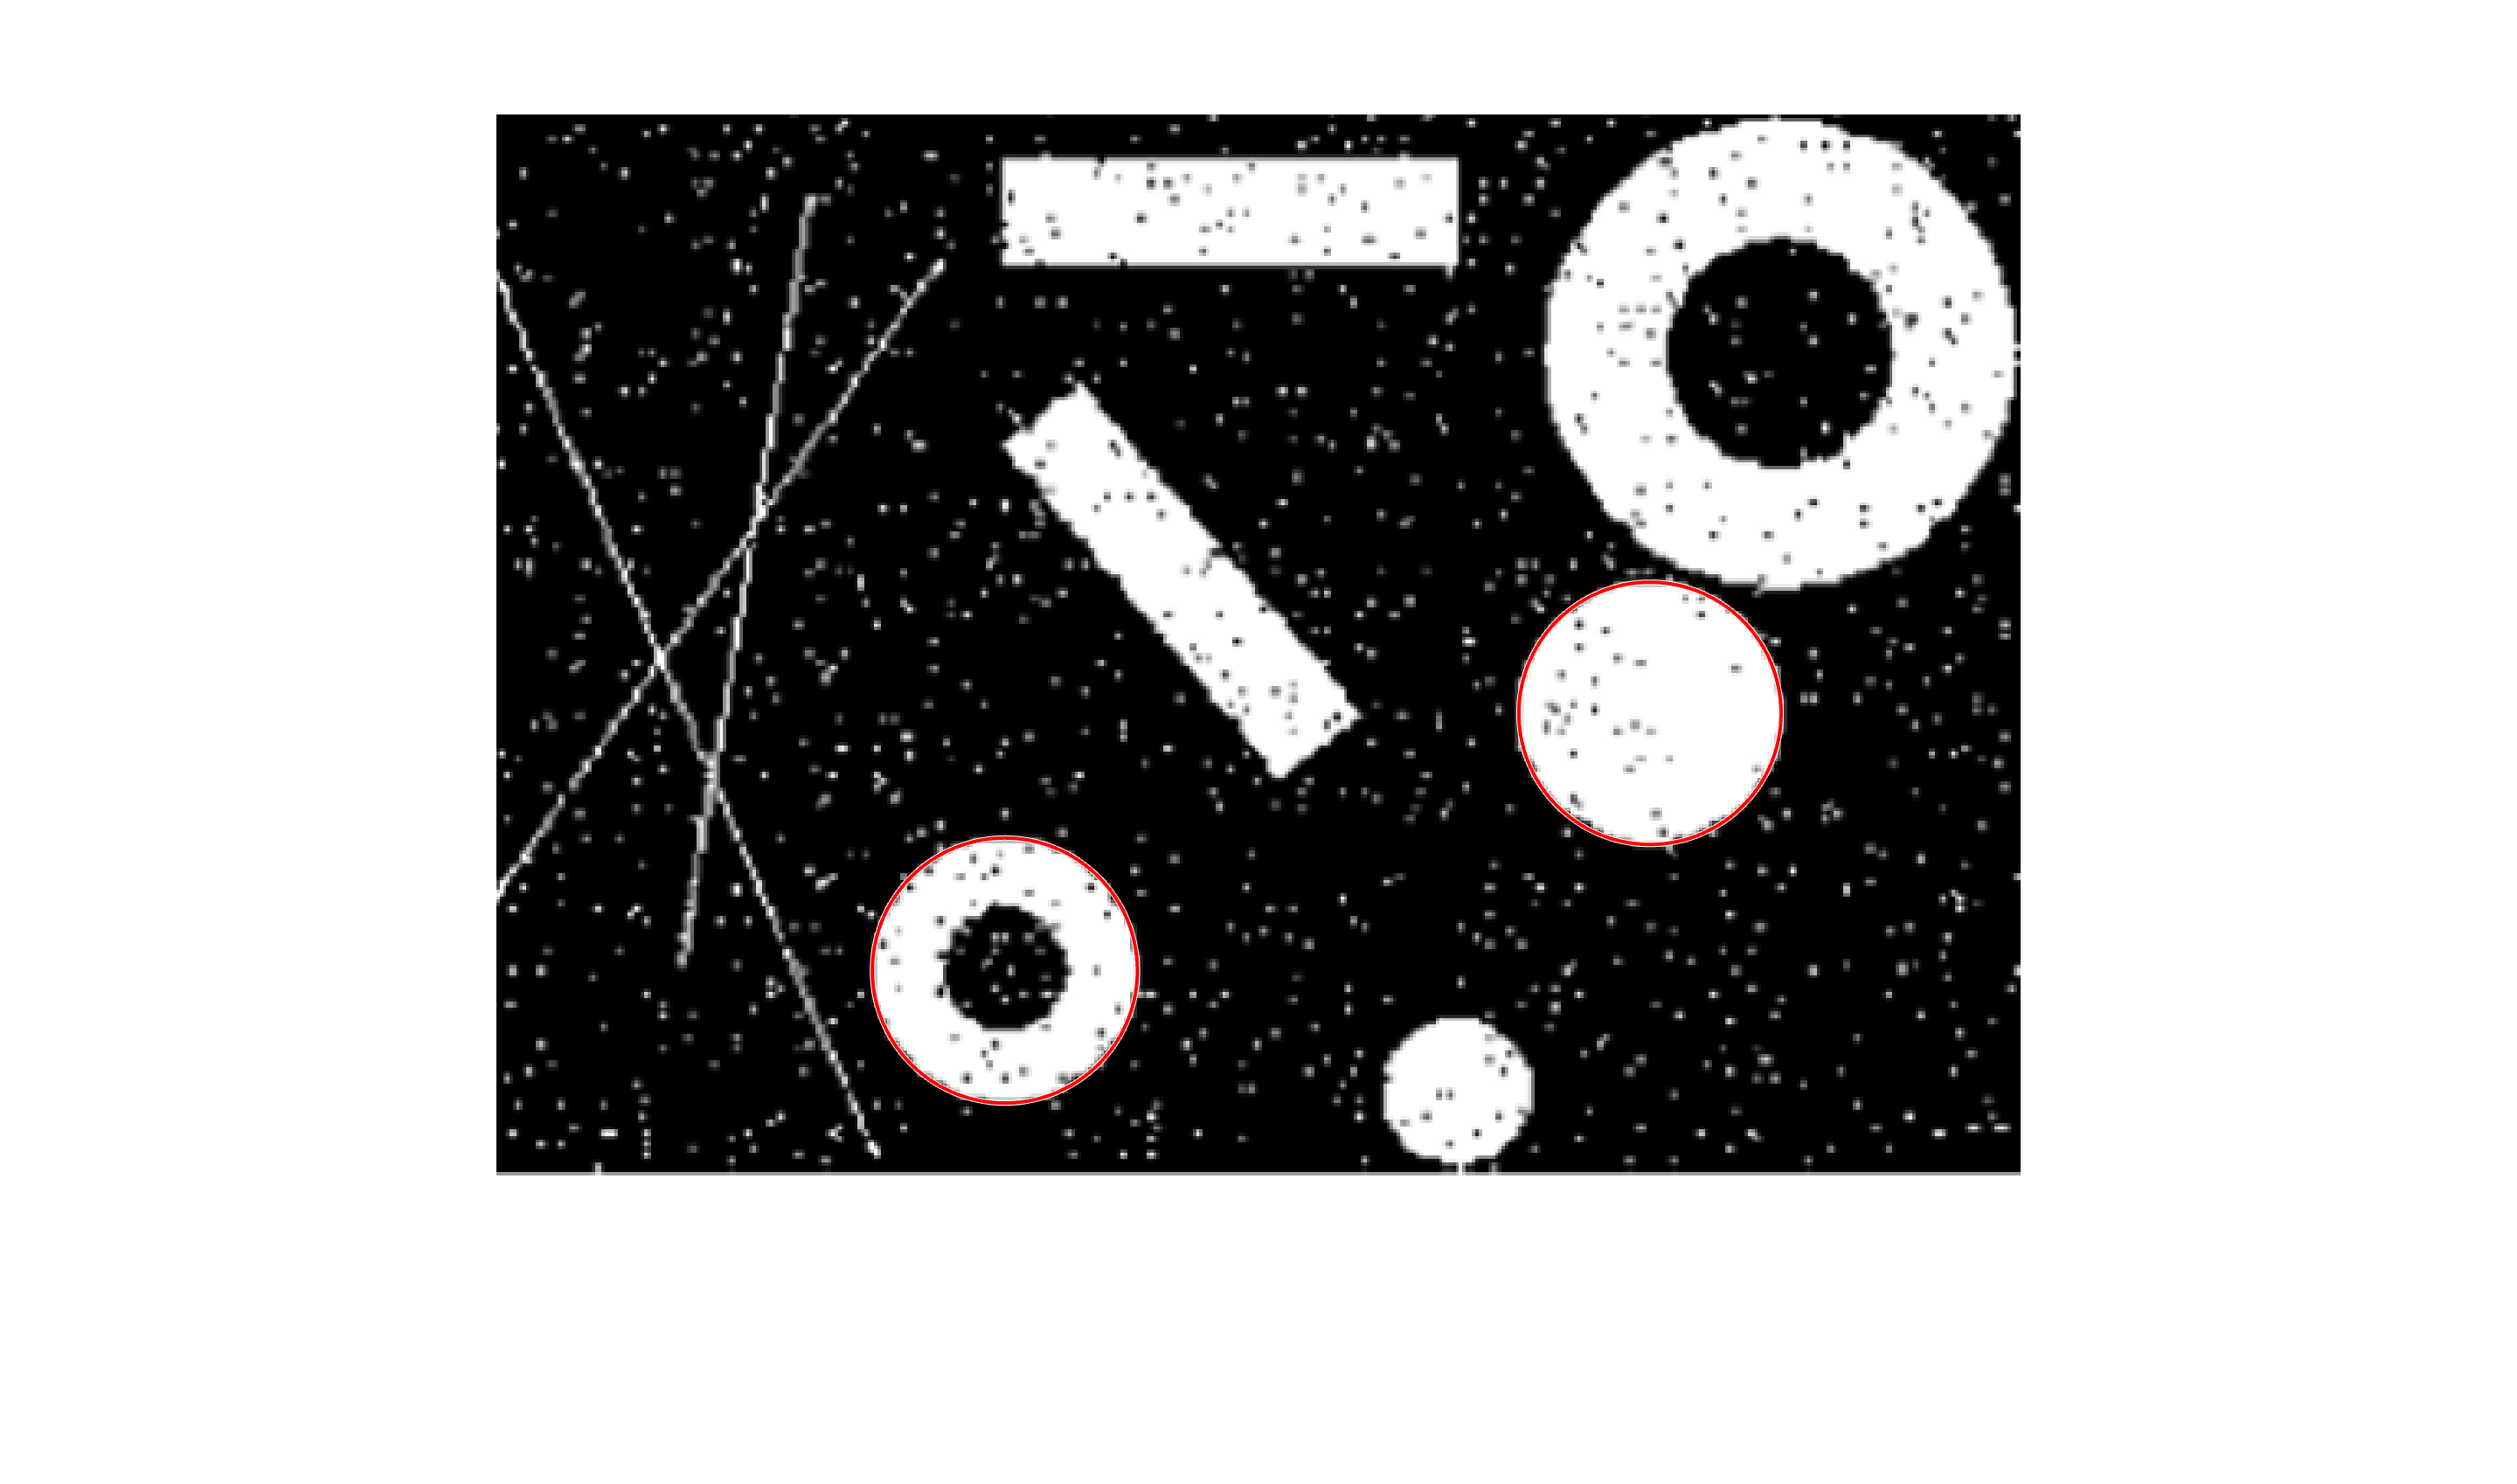
\includegraphics[width=9cm]{circle23.png} 	
	}
	\caption{圆与圆环检测结果2}
	\label{pic4}
\end{figure}
\begin{figure}[htbp]
	\centerline{
		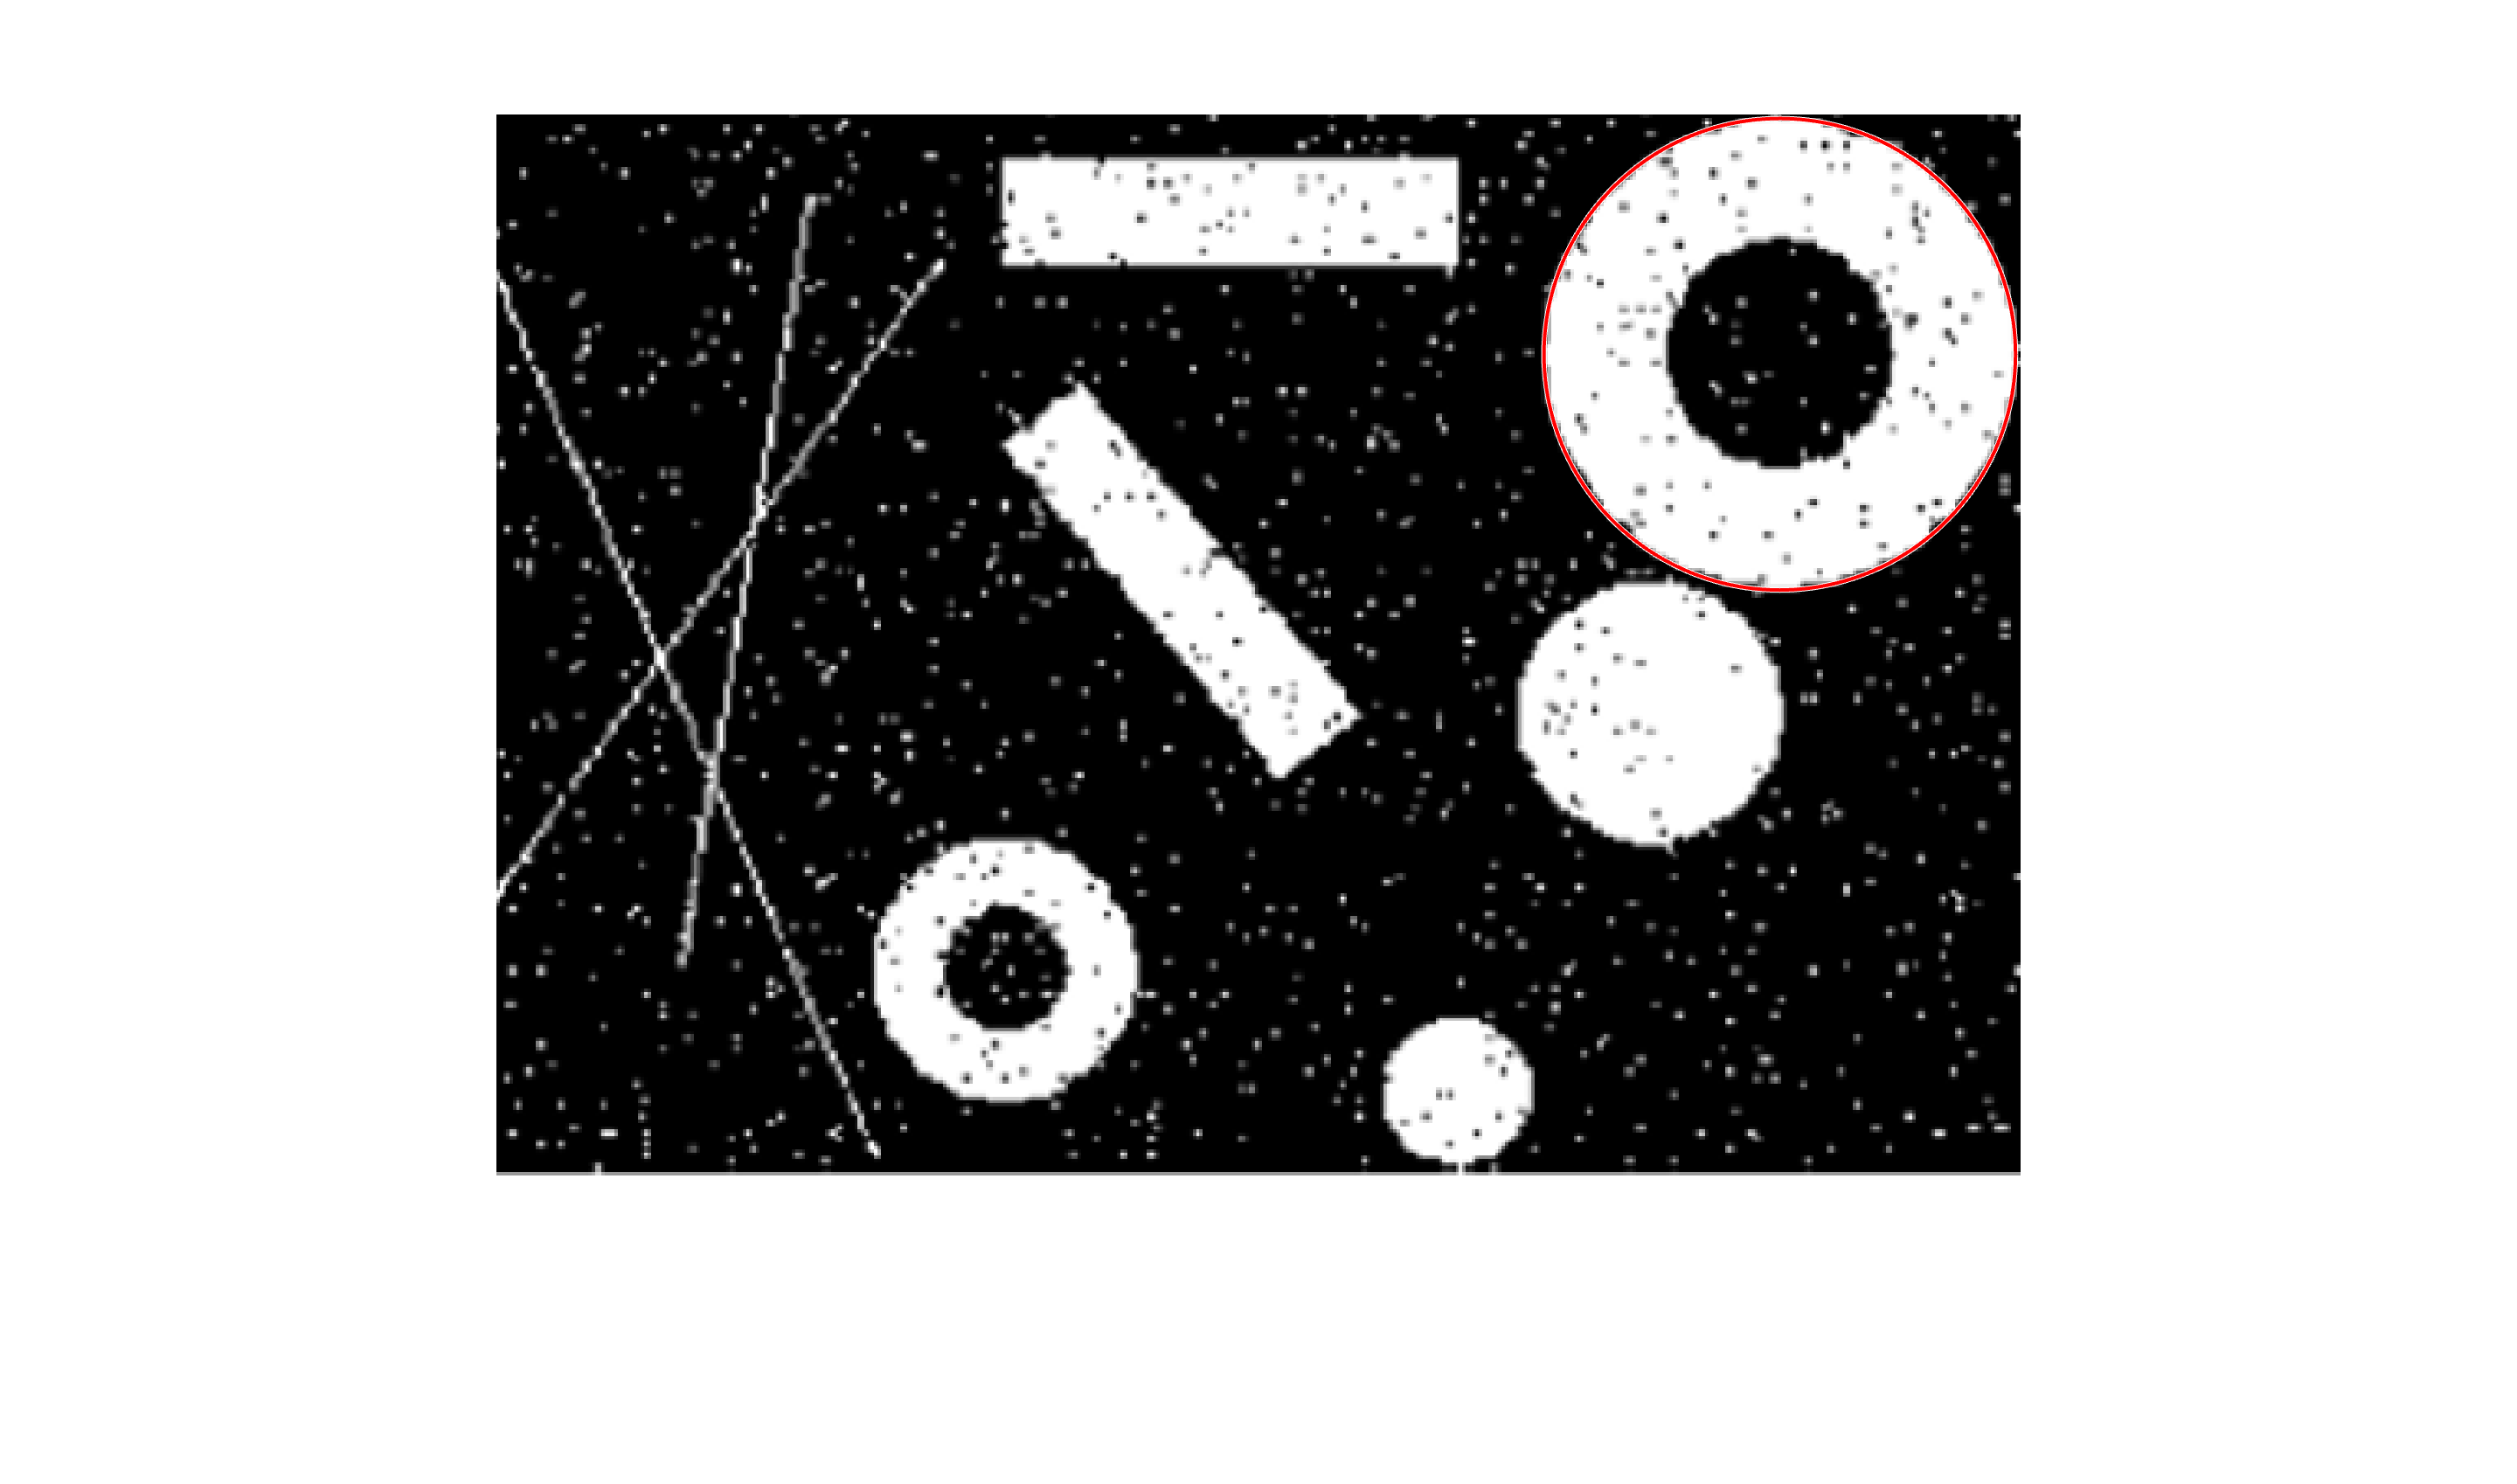
\includegraphics[width=9cm]{circle4.png} 	
	}
	\caption{圆与圆环检测结果3}
	\label{pic5}
\end{figure}
\begin{figure}[htbp]
	\centerline{
		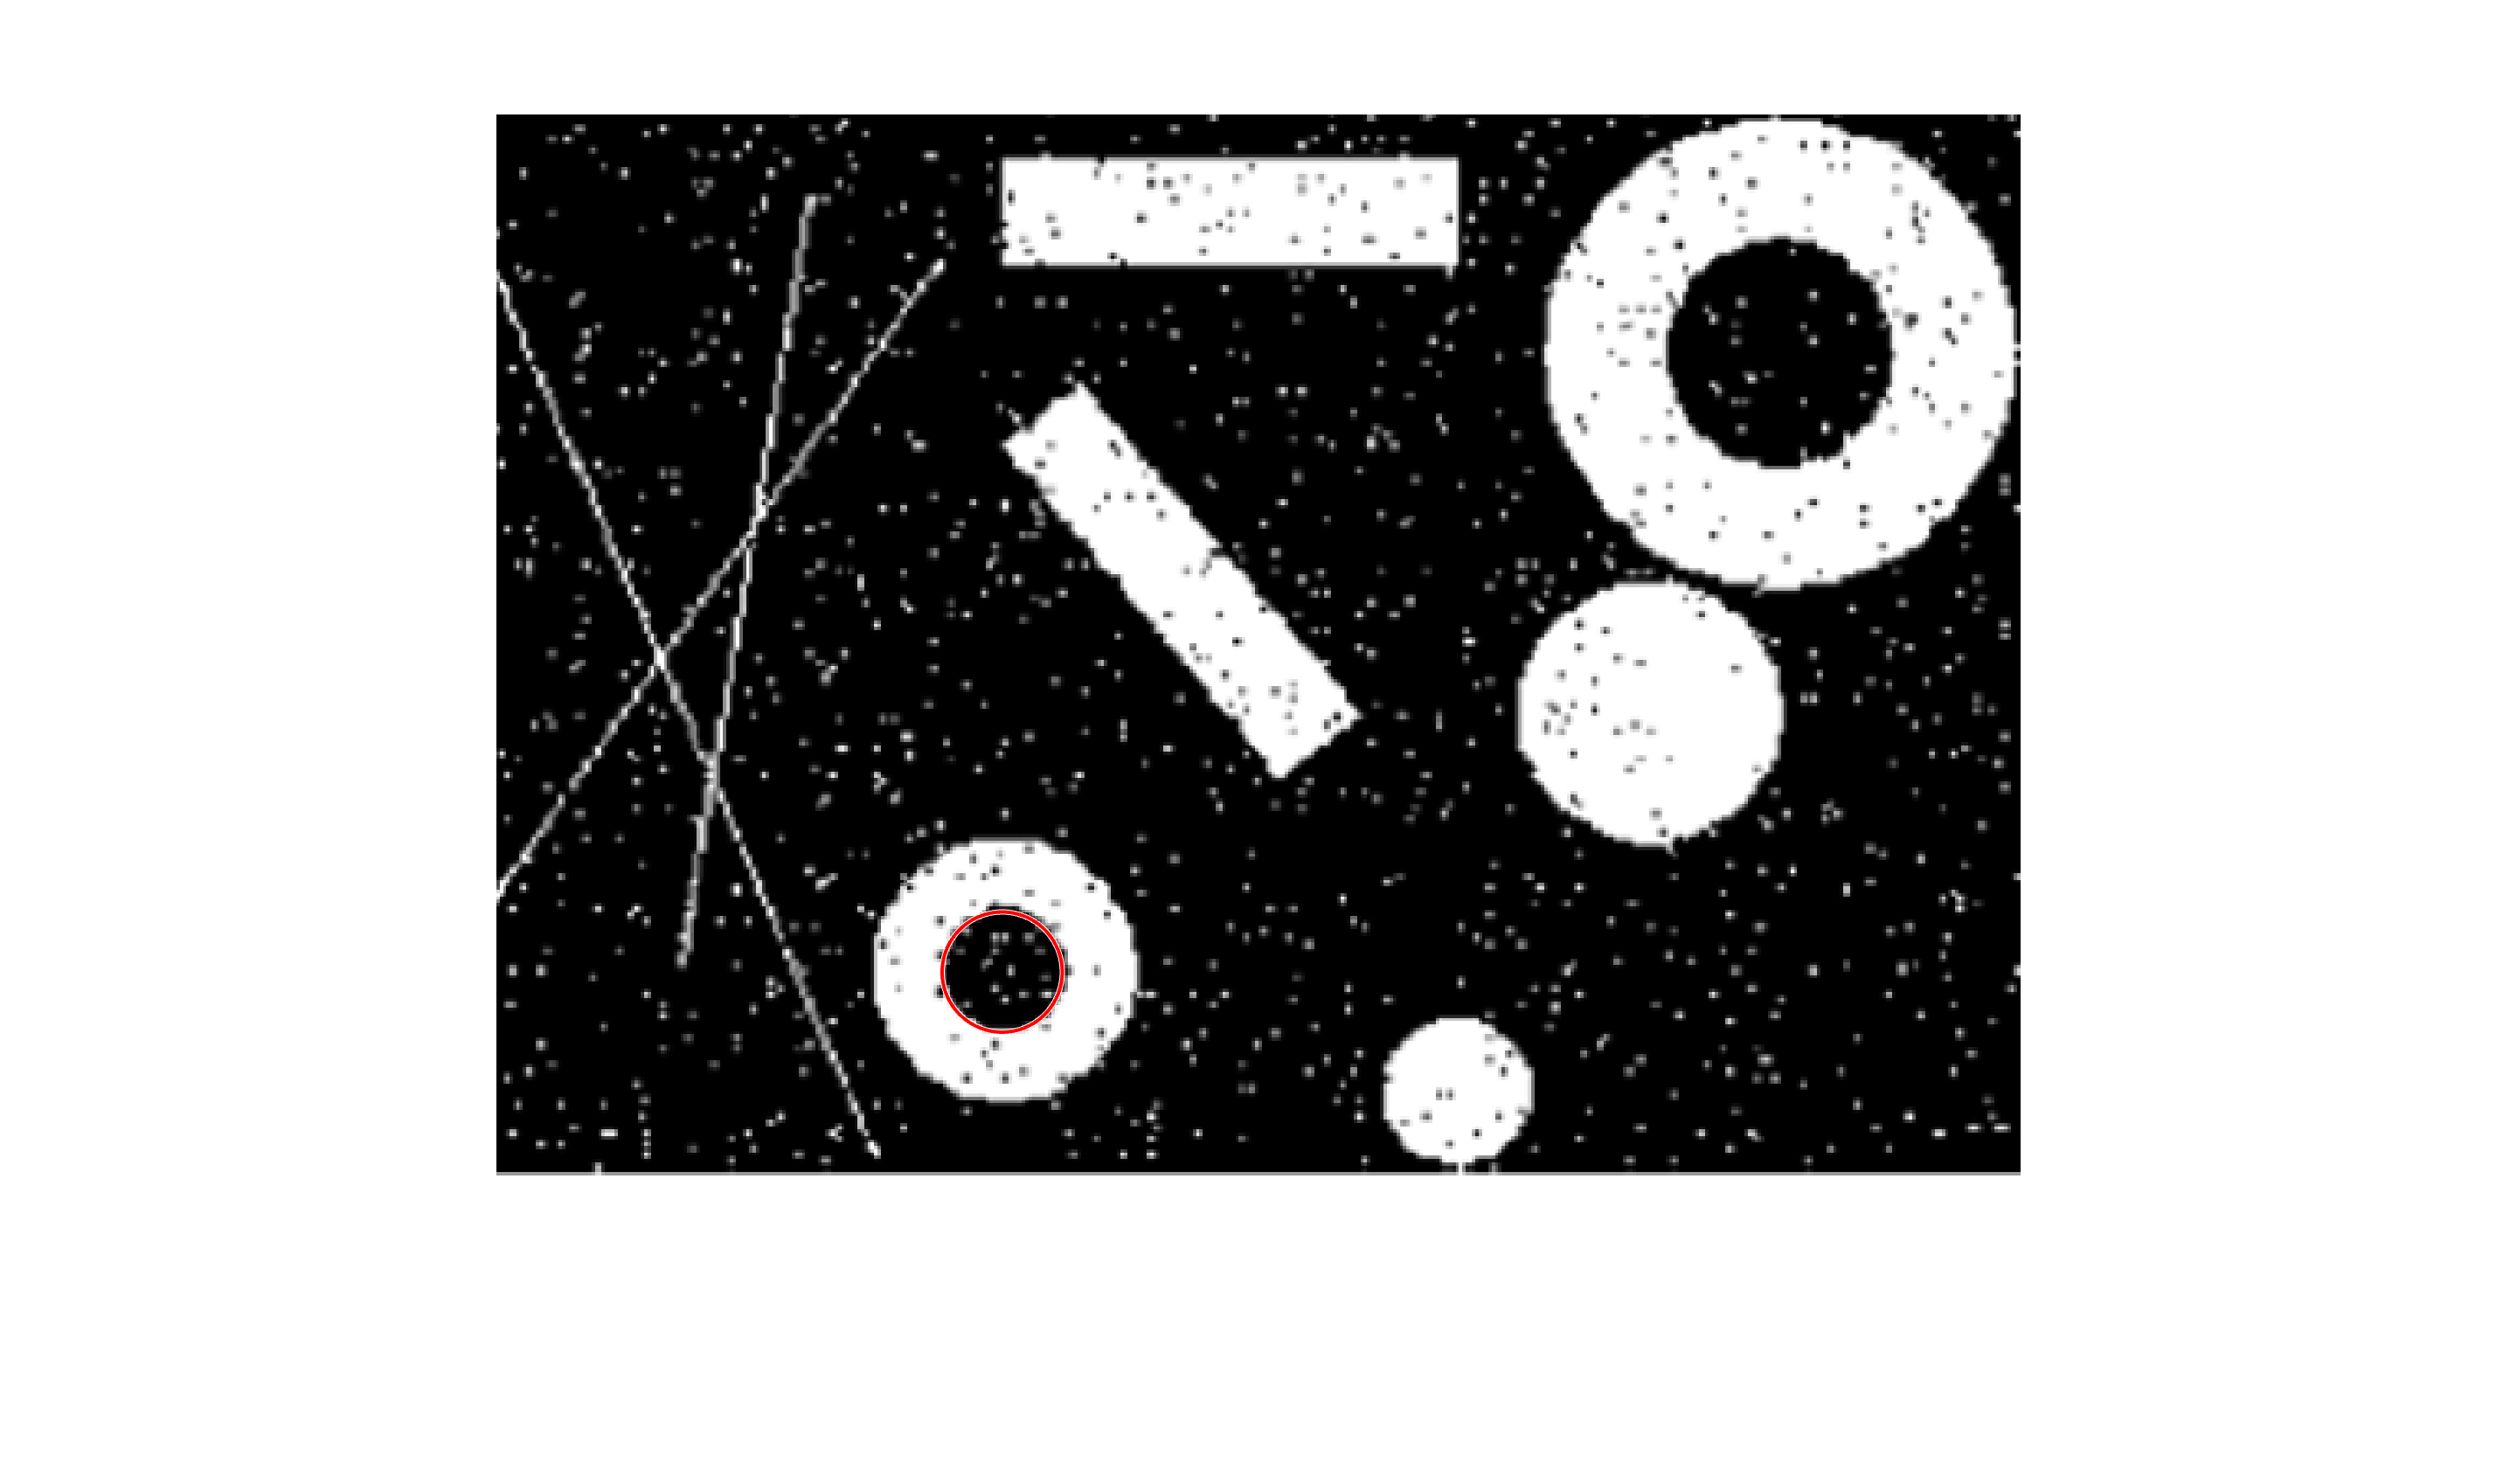
\includegraphics[width=9cm]{circle5.png} 	
	}
	\caption{圆与圆环检测结果4}
	\label{pic6}
\end{figure}
\begin{figure}[htbp]
	\centerline{
		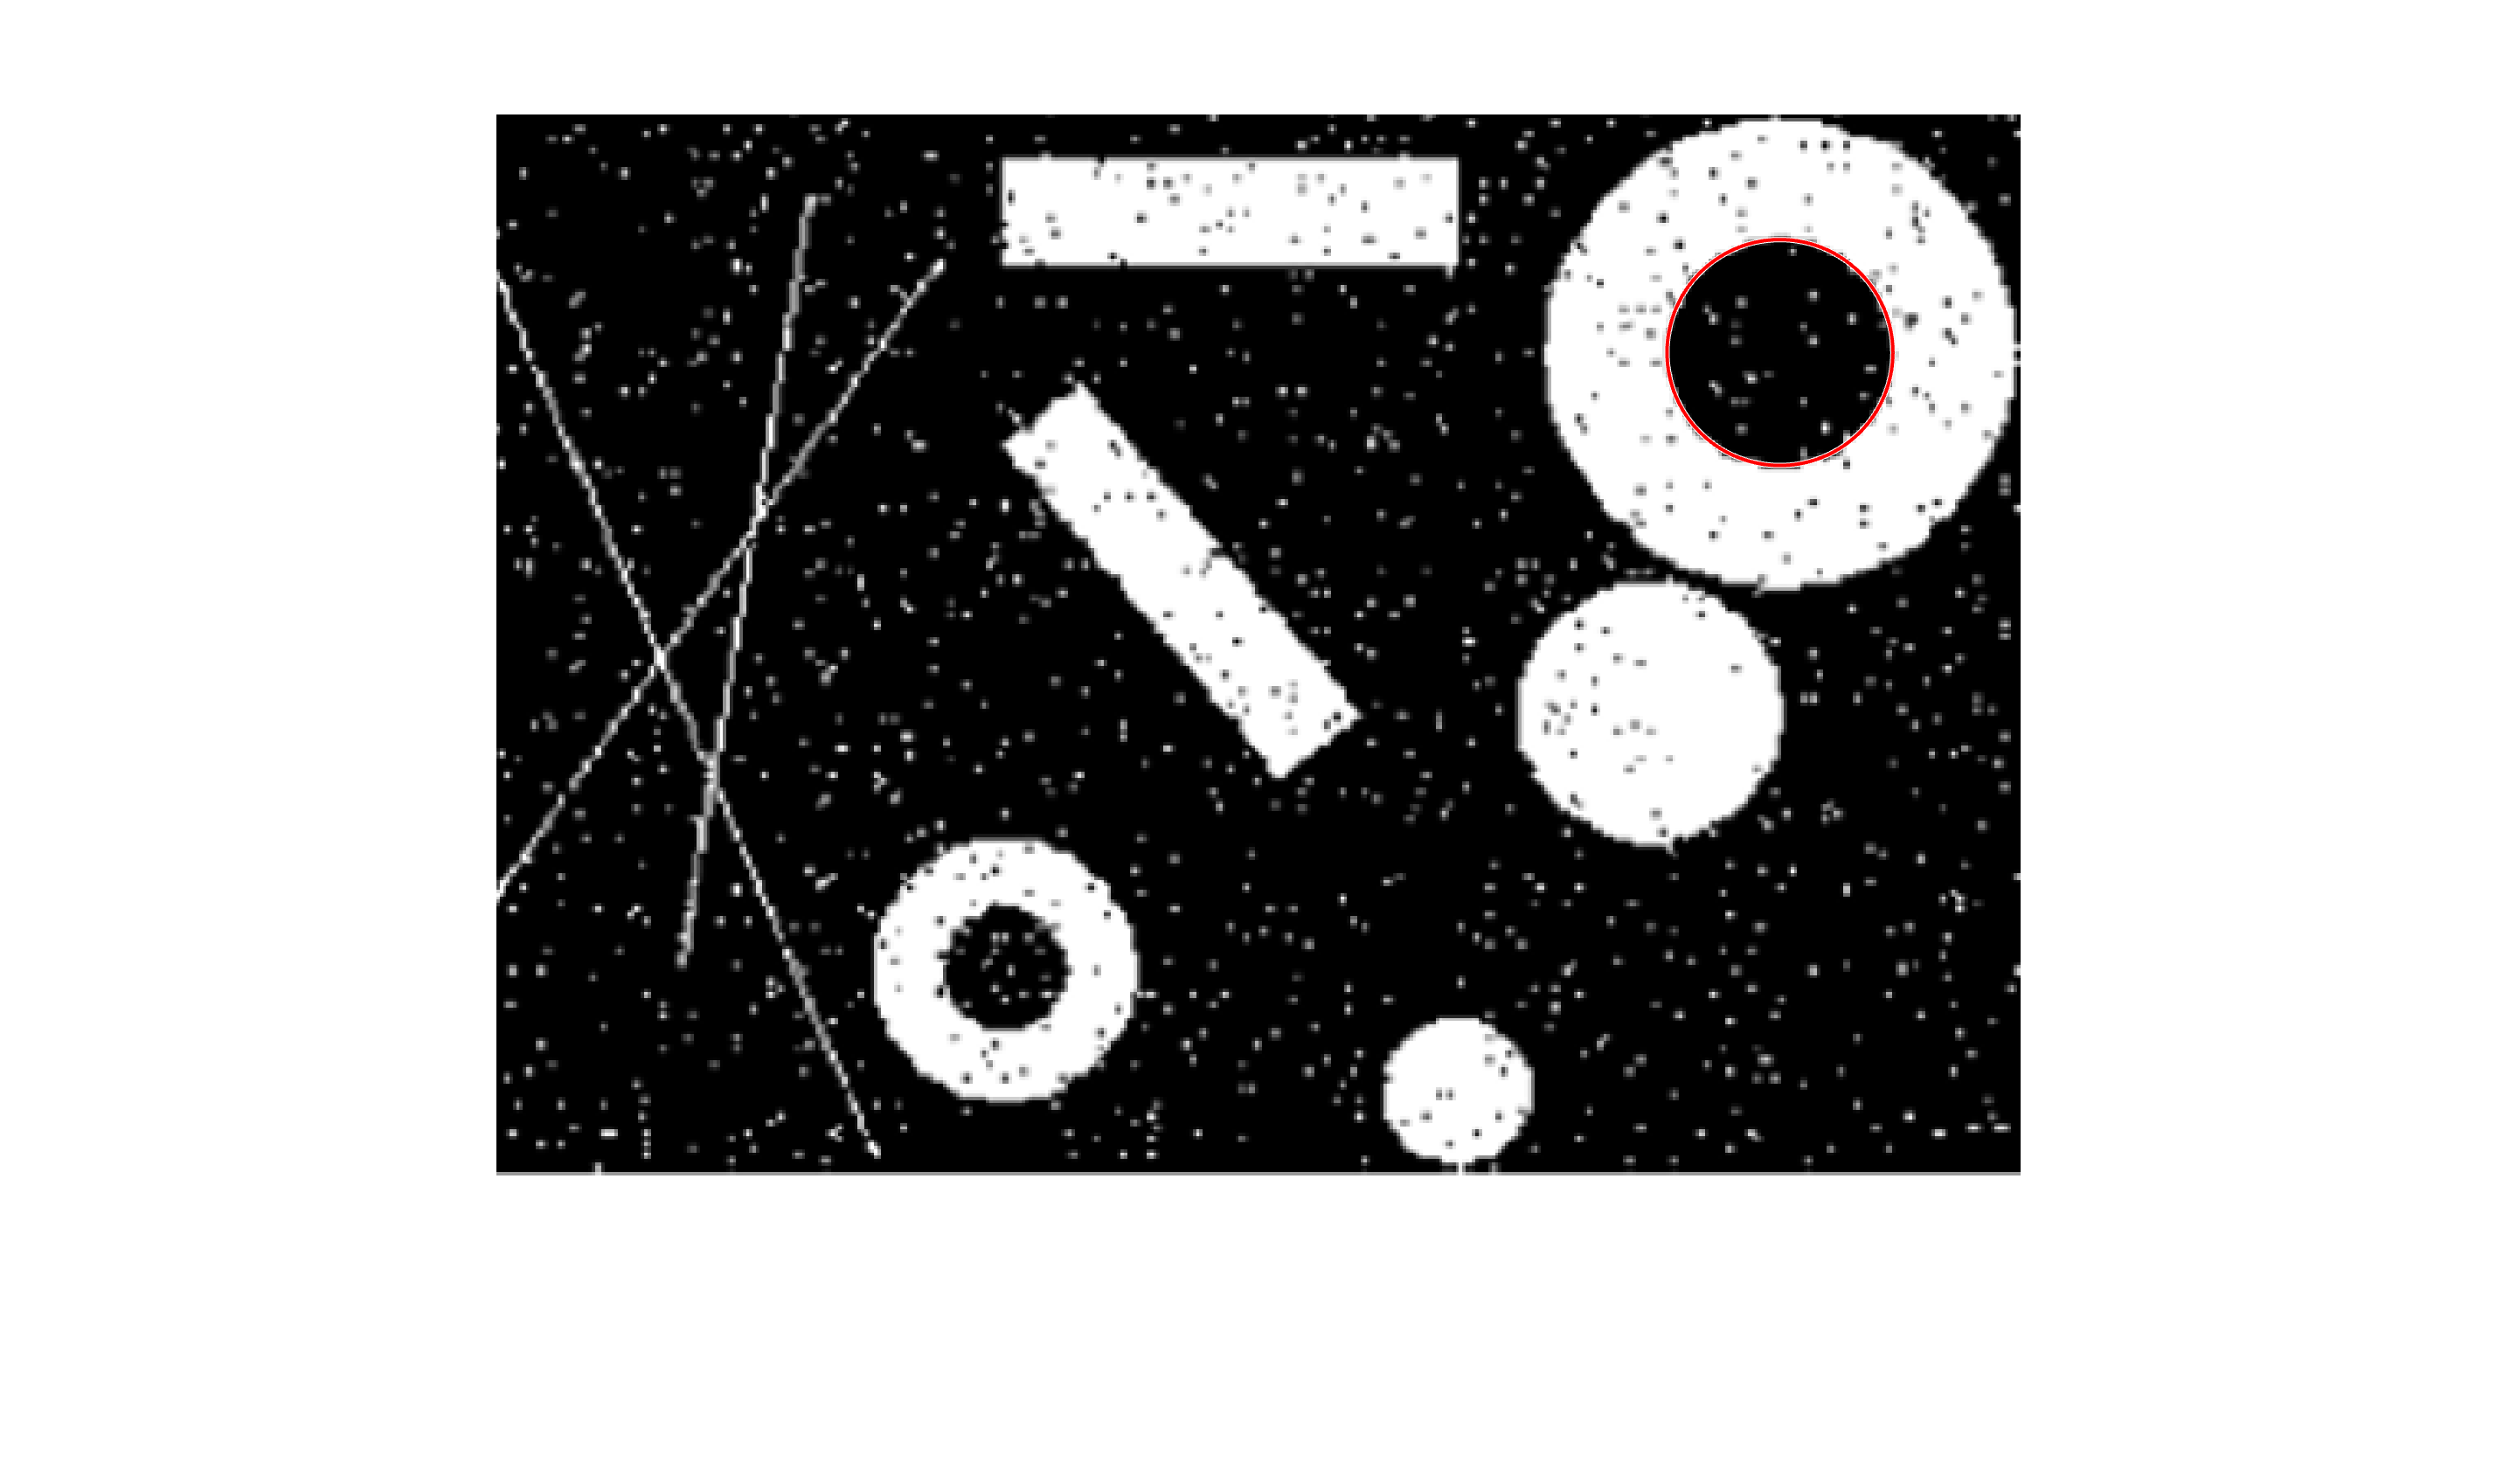
\includegraphics[width=9cm]{circle6.png} 	
	}
	\caption{圆与圆环检测结果5}
	\label{pic7}
\end{figure}

图片\ref{pic3}-\ref{pic7}显示了对灰度图像中圆与圆环进行识别与检测的结果。表格\ref{table2}给出了圆与圆环的半径与圆心坐标。
\begin{table}[htbp]
	\caption{圆与圆环检测结果}
	\label{table2} 
	\centering  
	\begin{tabular}{|c|c|c|}
	\hline
	圆/圆环 & 圆心坐标 & 半径 \\
	\hline
	圆1 & (293.7, 298.6)  & 22.8687 \\
	\hline
	圆2 & (351.7, 155.3) & 39.9 \\
	\hline
	圆环1(外环) & (182.8, 261.1)  & 40.3 \\
	\hline
	圆环1(内环) & (182.8, 261.1)  & 18.3 \\
	\hline
	圆环2(外环) & (391.2, 73.5)   & 71.8 \\
	\hline
	圆环2(内环) & (391.2, 73.5)   & 34.4 \\
	\hline
	\end{tabular}
\end{table}

\subsection{矩形检测结果}
\begin{figure}[htbp]
	\centerline{
		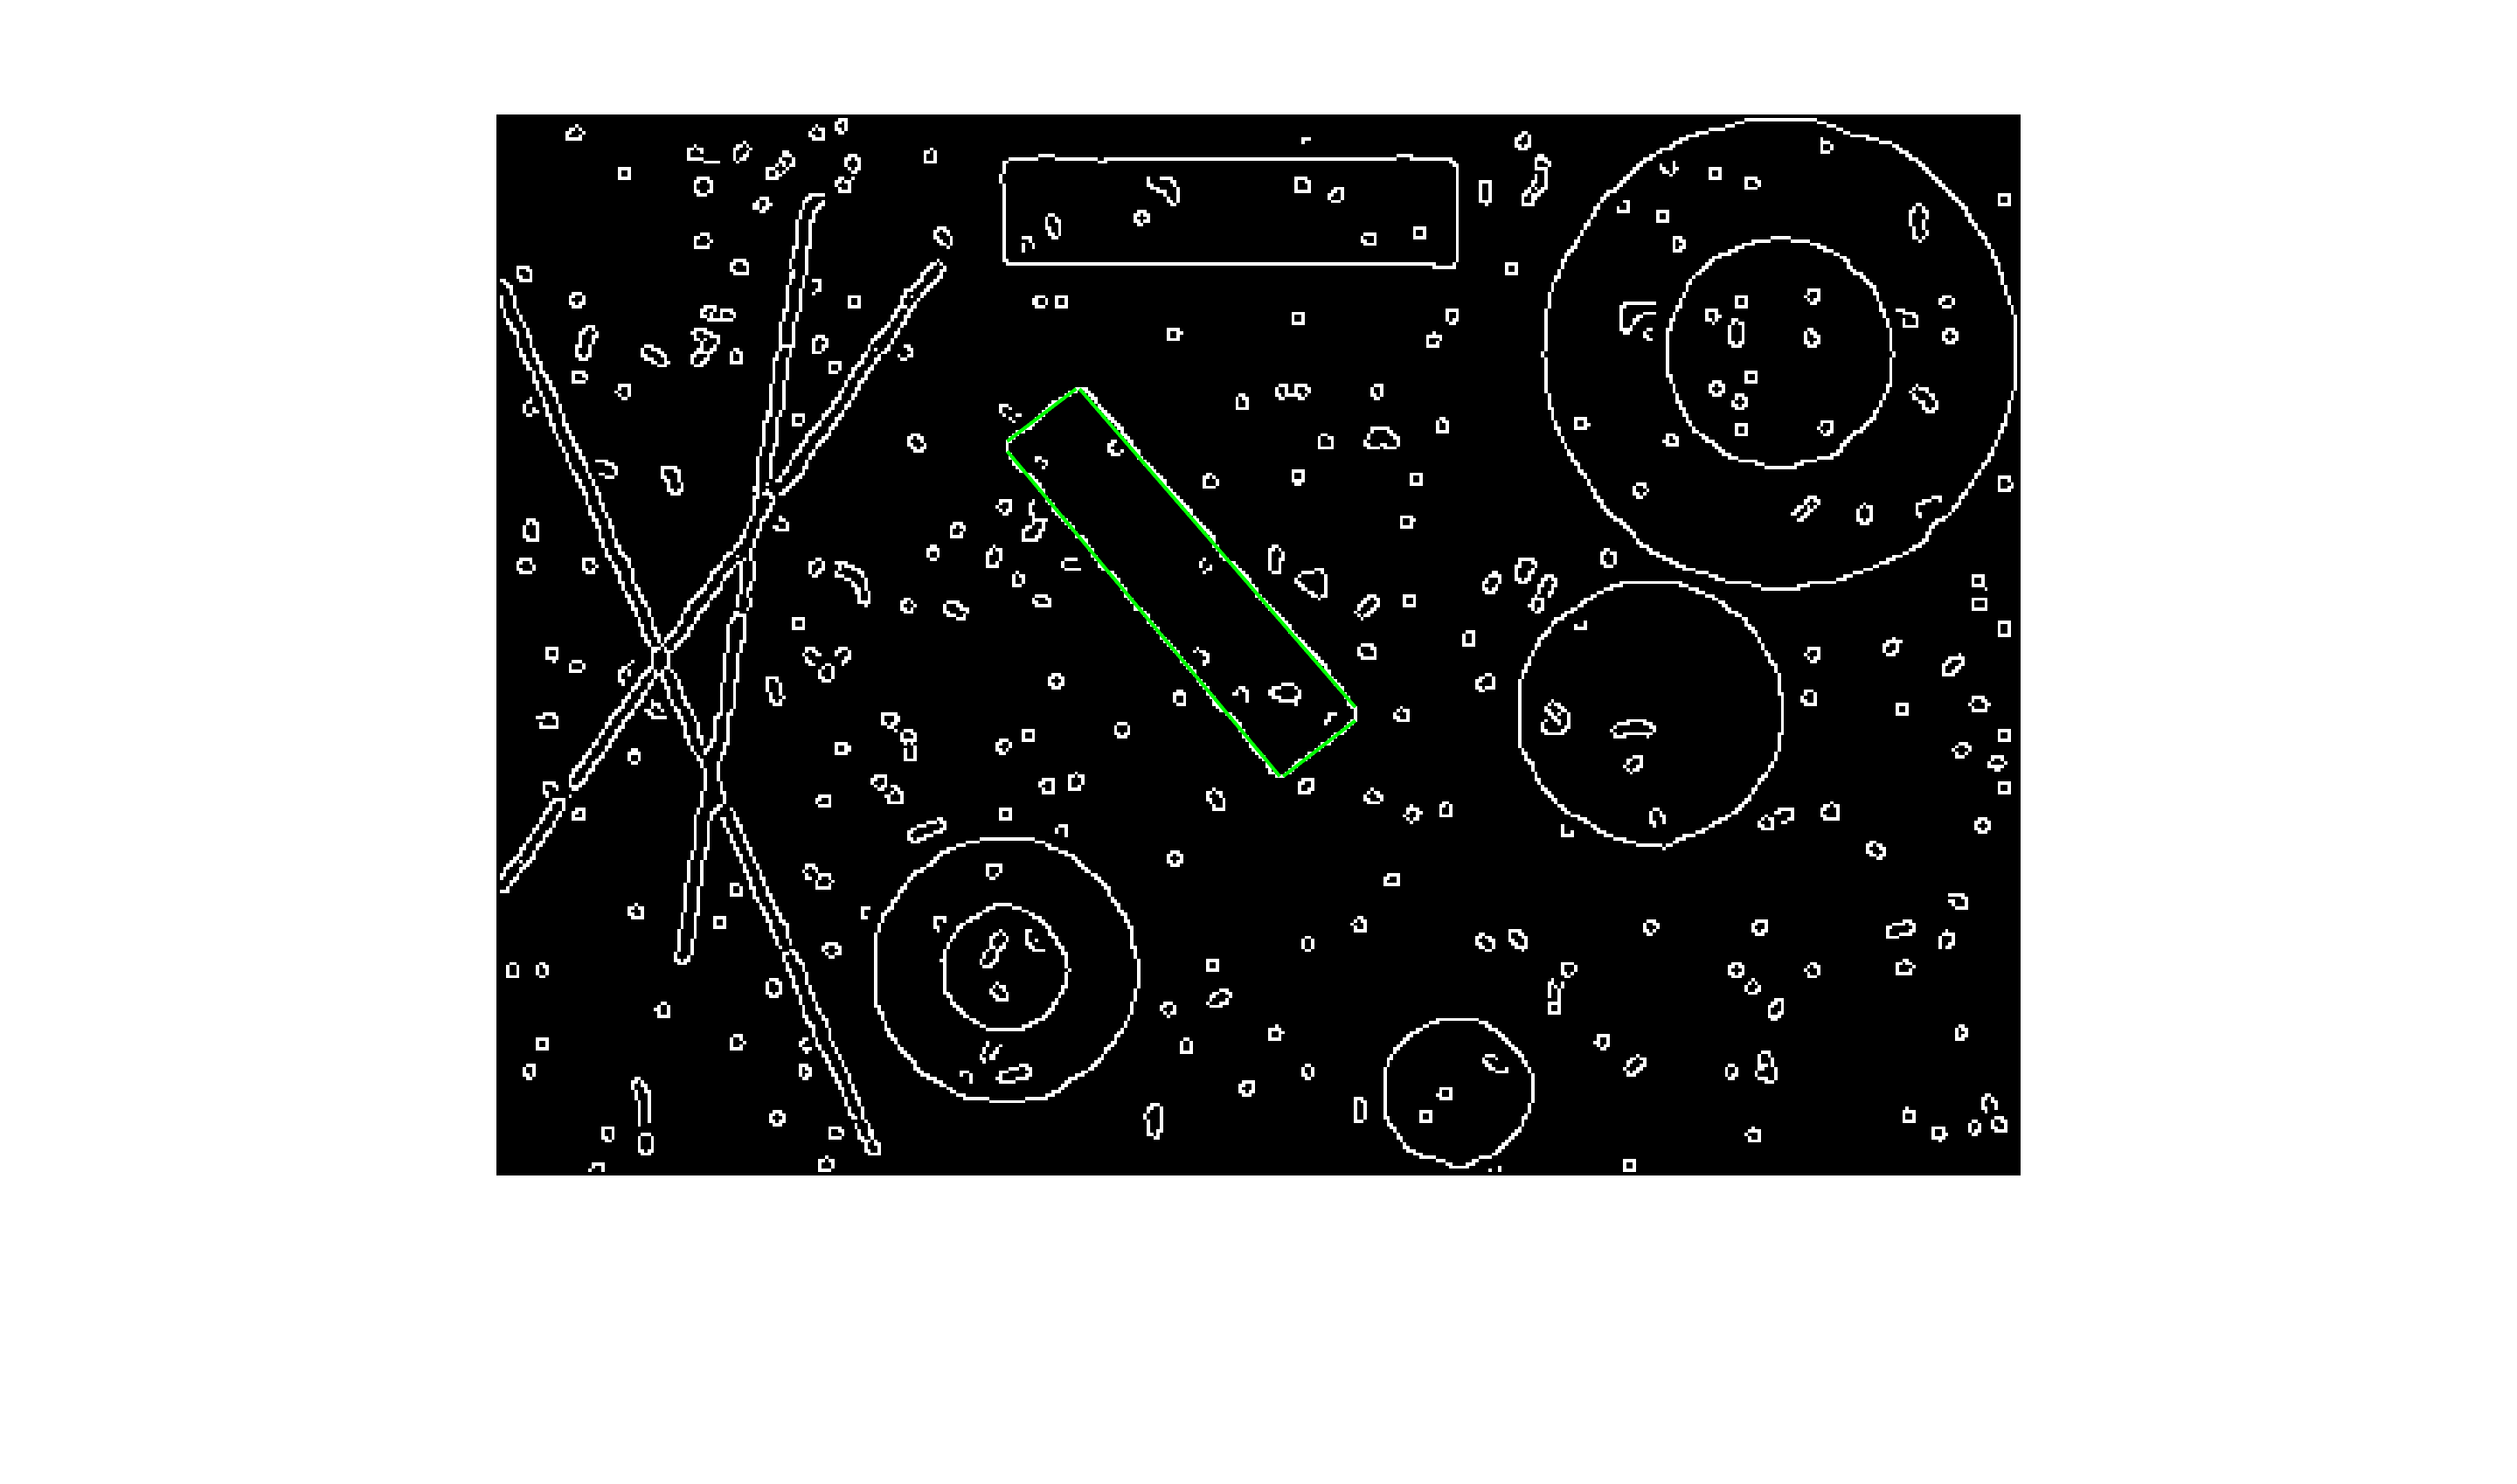
\includegraphics[width=9cm]{triangle1.png} 	
	}
	\caption{矩形检测结果1}
	\label{pic8}
\end{figure}
\begin{figure}[htbp]
	\centerline{
		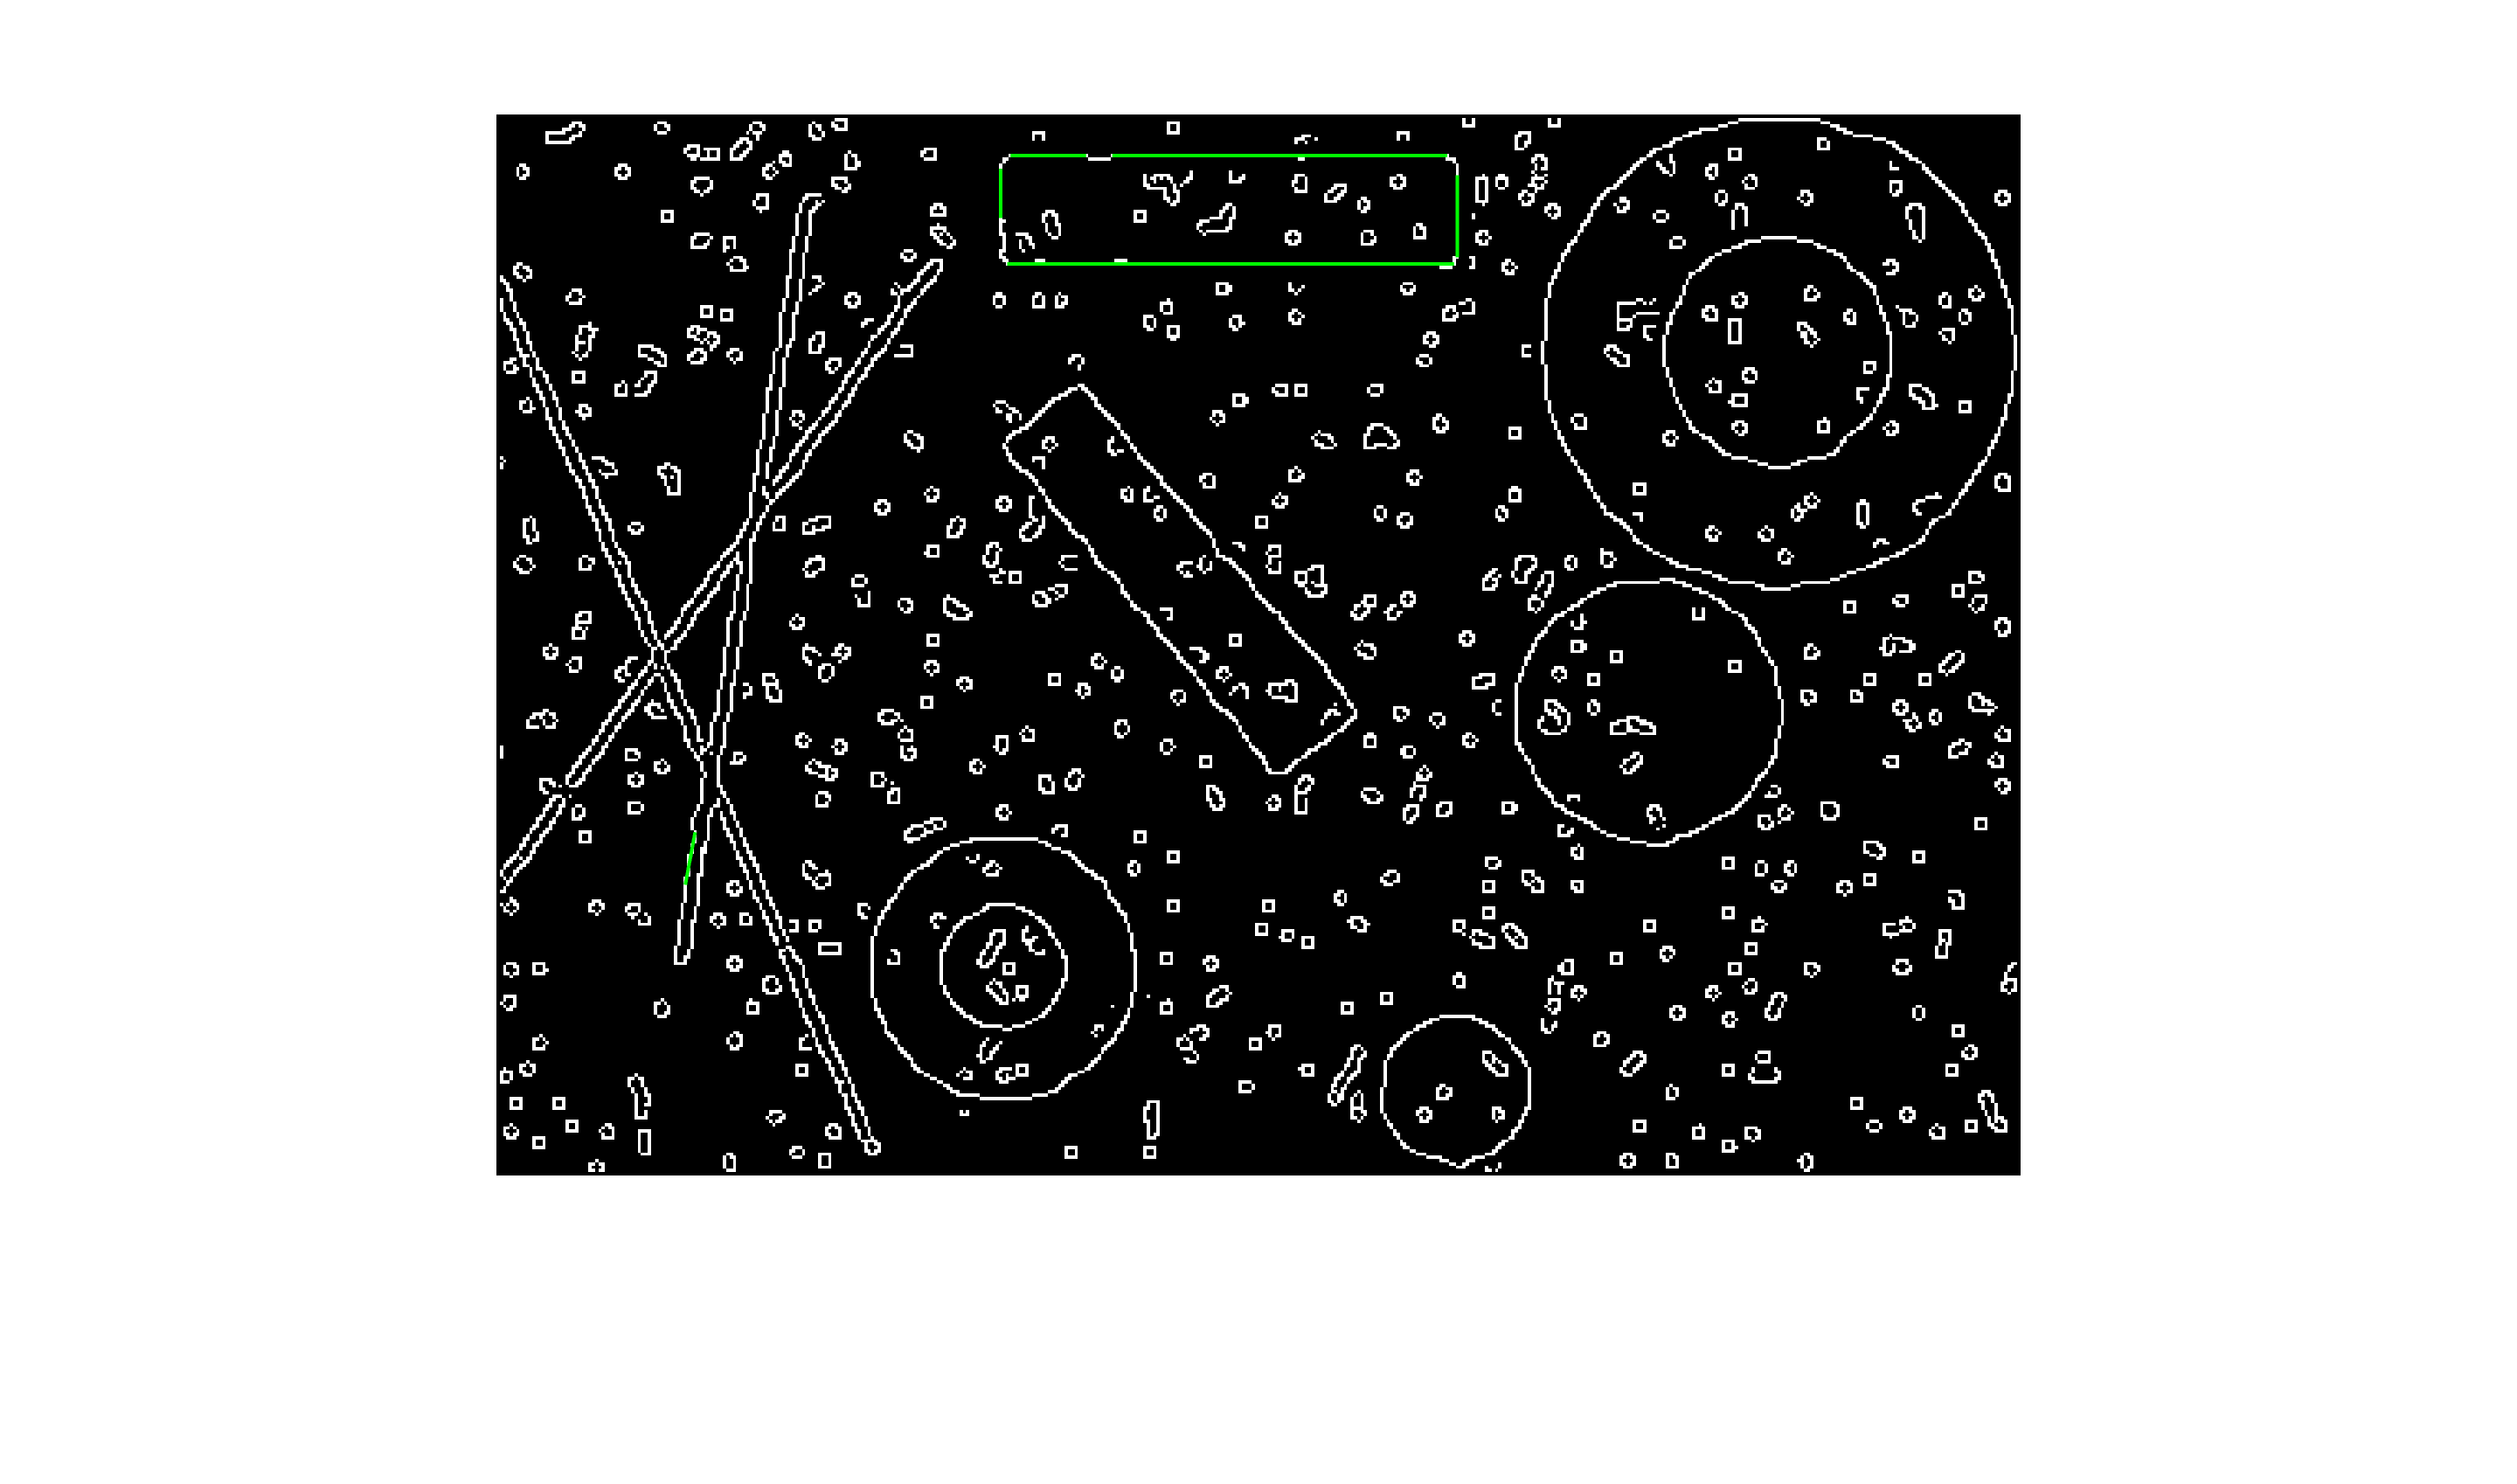
\includegraphics[width=9cm]{tri2.png} 	
	}
	\caption{矩形检测结果2}
	\label{pic9}
\end{figure}
图片\ref{pic8}与图片\ref{pic9}显示了对灰度图像中矩形进行识别与检测的结果。表格\ref{table3}给出了两个矩形的四个顶点坐标。

\begin{table}[htbp]
	\caption{矩形检测结果1}
	\label{table3} 
	\centering  
	\begin{tabular}{|c|c|c|c|c|}
	\hline
	矩形 & 顶点1 & 顶点2 & 顶点3 & 顶点4 \\
	\hline
	矩形1 & (178, 84)  & (262, 181) & (240, 202) & (156, 103) \\
	\hline
	矩形2 & (157, 13) & (290, 13) & (156, 46) & (292, 46) \\
	\hline
	\end{tabular}
\end{table}

\begin{table}[htbp]
	\caption{矩形检测结果2}
	\label{table4} 
	\centering  
	\begin{tabular}{|c|c|c|c|}
	\hline
	矩形 & 质心坐标 & 边长1 & 边长2 \\
	\hline
	矩形1 & (209, 142.5)  & 129.83 & 29.07 \\
	\hline
	矩形2 & (133, 13) & 223.5 & 29.5 \\
	\hline
	\end{tabular}
\end{table}

\section{总结}
本实践报告为数字图像处理课程中期实践报告,主要内容为图像目标检测。通过实际实践编程仿真加深了对图像处理的认识,同时学习并掌握了图像处理的基础知识。
\end{document}
